% %% %%%%%%%%%%%%%%%%%%%%%%%%%%%%%%%%%%%%%%%%%%%%%%%%%%%%%%%%%%
% step-1.tex
%
% Author:  Mauricio Matamoros
% License: MIT
%
% %% %%%%%%%%%%%%%%%%%%%%%%%%%%%%%%%%%%%%%%%%%%%%%%%%%%%%%%%%%%
%!TEX root = ../practica.tex
%!TEX root = ../references.bib

% CHKTEX-FILE 1
% CHKTEX-FILE 13
% CHKTEX-FILE 46

\subsection{Paso 1: Alambrado}%
\label{sec:step1}

El proceso de alambrado de esta práctica considera dos circuitos.
El primer circuito (véase \Cref{fig:circuit-ac}) opera con corrente alterna e integra un detector de cruce por cero y un convertidor AC-AC con base en un TRIAC.
Ambos subcircuitos cuentan con optoacopladores que servirán como interfaz para una conexión segura al circuito de DC.

El segundo circuito (véase \Cref{fig:circuit-dc}) está encargado de detectar el cruce por cero y enviar la señal de activación al TRIAC en el momento oportuno de acuerdo con la potencia requerida por el usuario (el brillo del foco) mediante una interfaz gráfica.

\medskip
\begin{importantbox}{\large \textsc{Advertencia}}
	\begin{center}
		Asegúrese de que todos los cables para el circuito AC están perfectamente aislados.

		Las puntas expuestas son un riesgo de electrocución y quemarán su arduino y su Pi con un sólo roce.

		\medskip{}

		\textbf{Utilice cinta aislante.}
	\end{center}
\end{importantbox}

Para este fin, se alambra la señal del subcircuito detector de cruce por cero a un pin te interrupción del Arduino que iniciará un \emph{timer} en hardware y enviará la señal de activación al TRIAC una vez que transcurra el tiempo de activación para obtener así la potencia deseada.
Asimismo, el Arduino recibirá via \IIC de la Raspberry Pi la potencia solicitada por el usuario mediante una interfaz web.

Cabe mencionar que, al ser un circuito completamente digital, al GPIO de la Raspberry Pi podría configurársele un pin en modo interrupción para recibir la señal del detector de cruce por cero y otro para el envío de la señal de activación del TRIAC.
Sin embargo, el paquete \texttt{RPi.GPIO} para el control de la GPIO con Python no soporta el uso de interrupciones de timer en hardware, por lo que no es posible garantizar que la señal de activación del TRIAC será enviada sin retrasos.
Es por este motivo que se utiliza un Arduino como auxiliar.

\subsubsection{Circuito de potencia en AC}%
Alambre primero el circuito de corriente alterna de la \Cref{fig:circuit-ac} tras verificar los valores de las resistencias de los optoacopladores.
Considere que si la resistencia de gatillo es muy grande (ej. 10M$\Omega$), el optoacoplador no recibirá suficente corriente y no encenderá lo suficiente como para disparar el fotosensor.
Por otro lado, si la resistencia es demasiado pequeña el optoacoplador se quemará irremediablemente.

\begin{figure}[H]
	\centering
	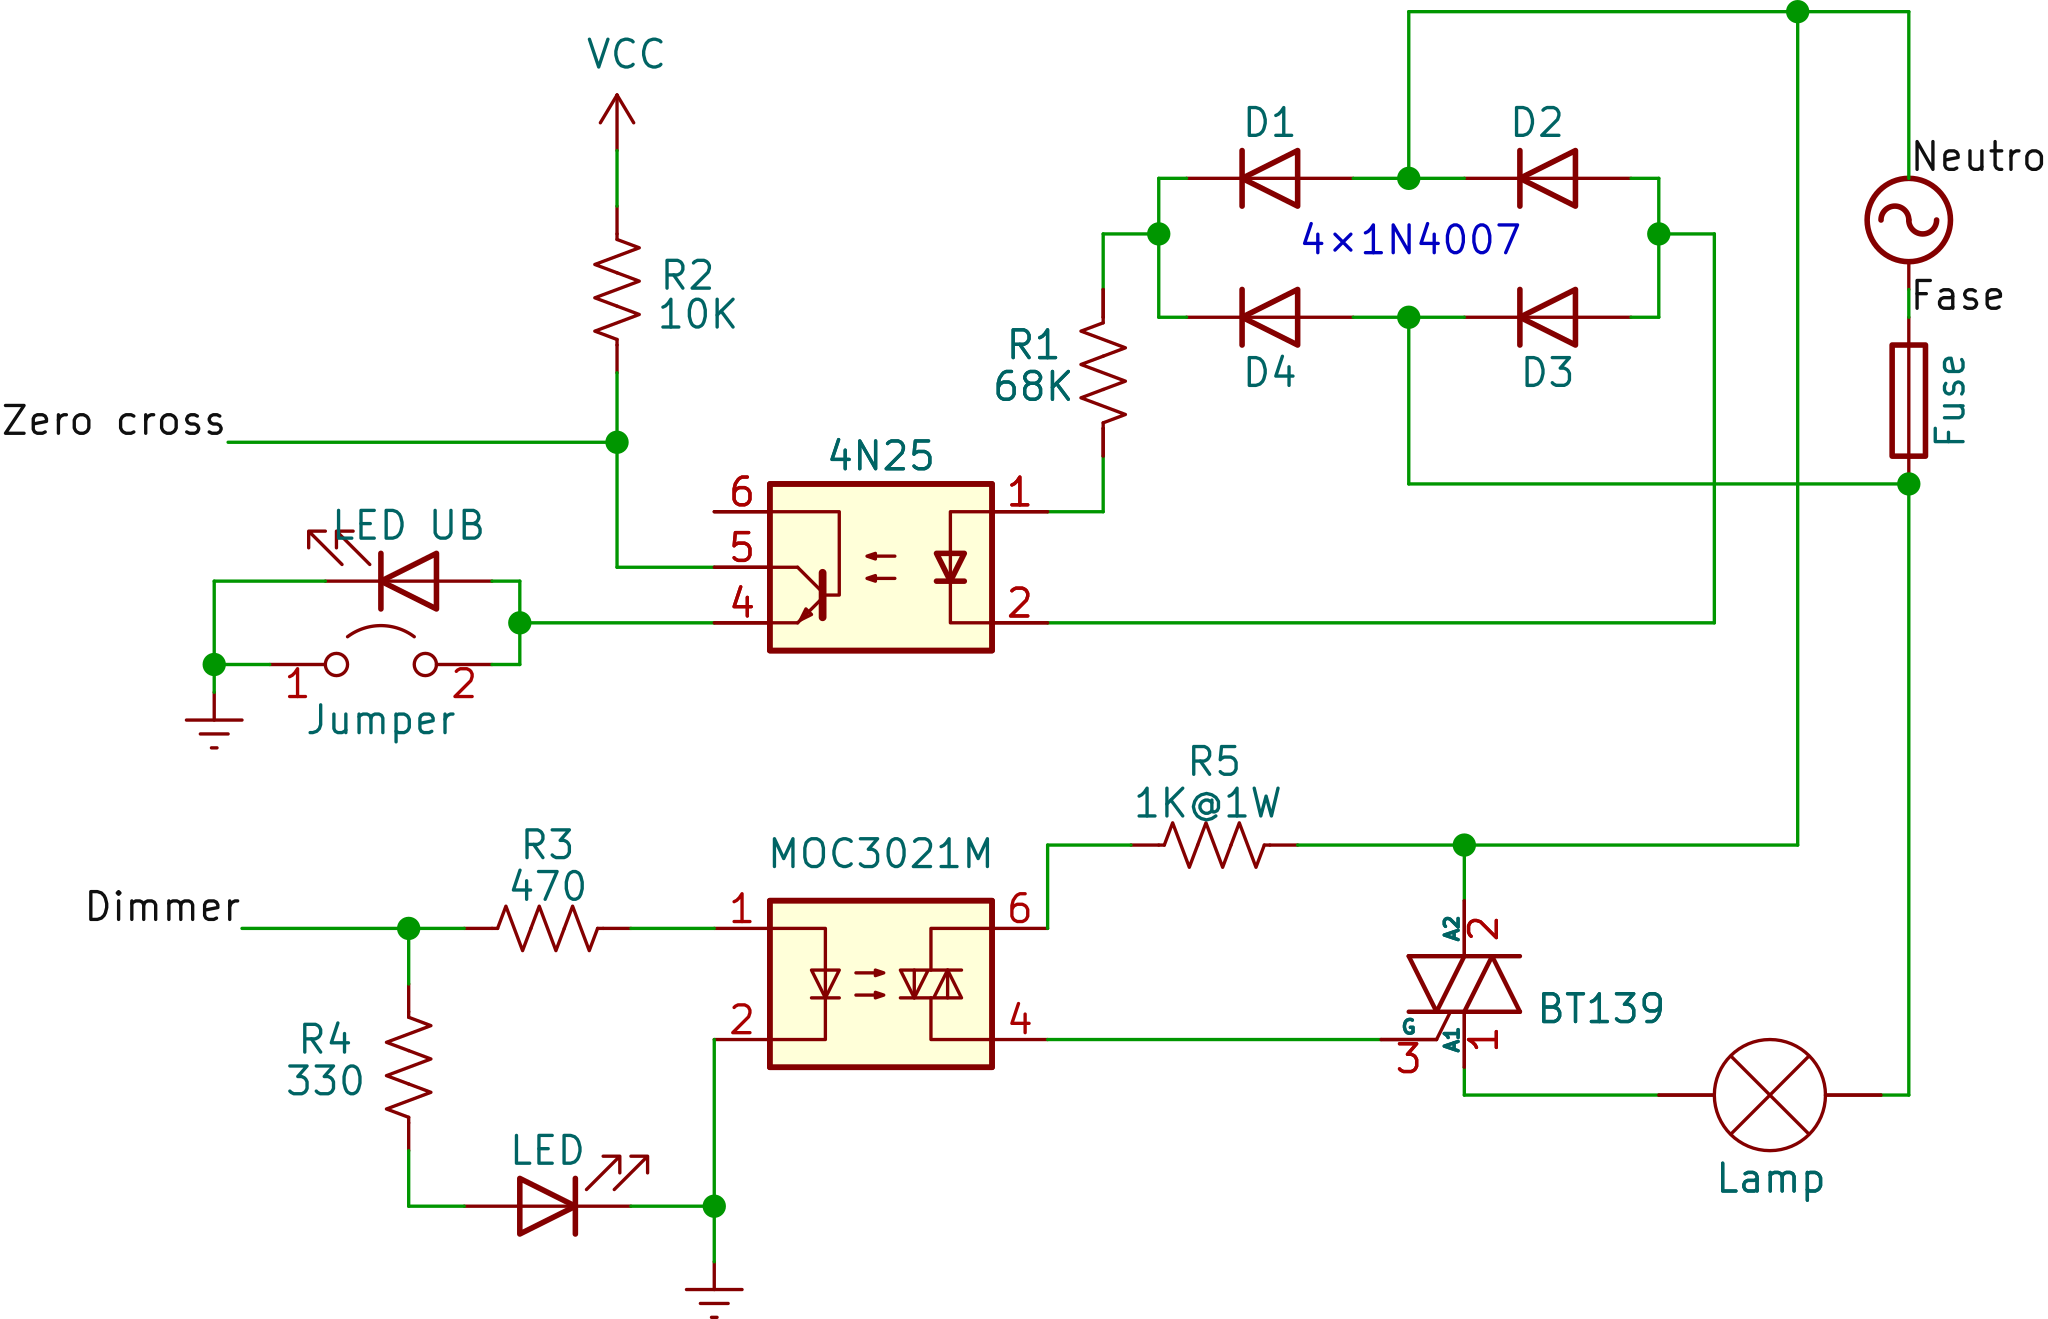
\includegraphics[width=0.5\columnwidth,height=7cm,keepaspectratio]{img/circuit-ac.png}
	\caption{Circuito de potencia en AC}%
	\label{fig:circuit-ac}
\end{figure}

Tras alambrar el circuito, es una buena idea probar el detector de cruce por cero con un osciloscopio, o al menos con un led ultrabrillante (LED UB), que deberá encender tenuemente.
De igual manera, conviene probar el encendido del foco inyectando 5V al MOC que acopla al TRIAC.

\medskip
\begin{importantbox}{\large Importante}
	\begin{center}
		Asegúrese de verificar con un multímetro que el circuito de AC está debidamente aislado y que no se tienen valores mayores a 5V en el segmento de DC.
		De otro modo podría quemar su Arduino y su Raspberry Pi.
	\end{center}
\end{importantbox}

Continúe el alambrado del circuito.

\subsubsection{Circuito de control en DC}%
Alambre el circuito de corriente directa de la \Cref{fig:circuit-dc} tras verificar la tensión de las señales optoacopladas conectando el bus \IIC entre la Raspberry Pi y el Arduino como ilustran la \Cref{tbl:pi-arduino-i2c} y la \Cref{fig:circuit-dc}.
Hay tutoriales que sugieren utilizar un convertidor de niveles de voltaje cuando se conecta una Raspberry Pi a un arduino mediante \IIC, especialmente cuando la Raspberry Pi opera a 3.3V.
Esto \textbf{NO} es necesario si la Raspberry Pi está configurada como dispositivo maestro o \emph{master} y el Arduino como dispositivo esclavo o \emph{slave}.

\begin{figure}[H]
	\centering
	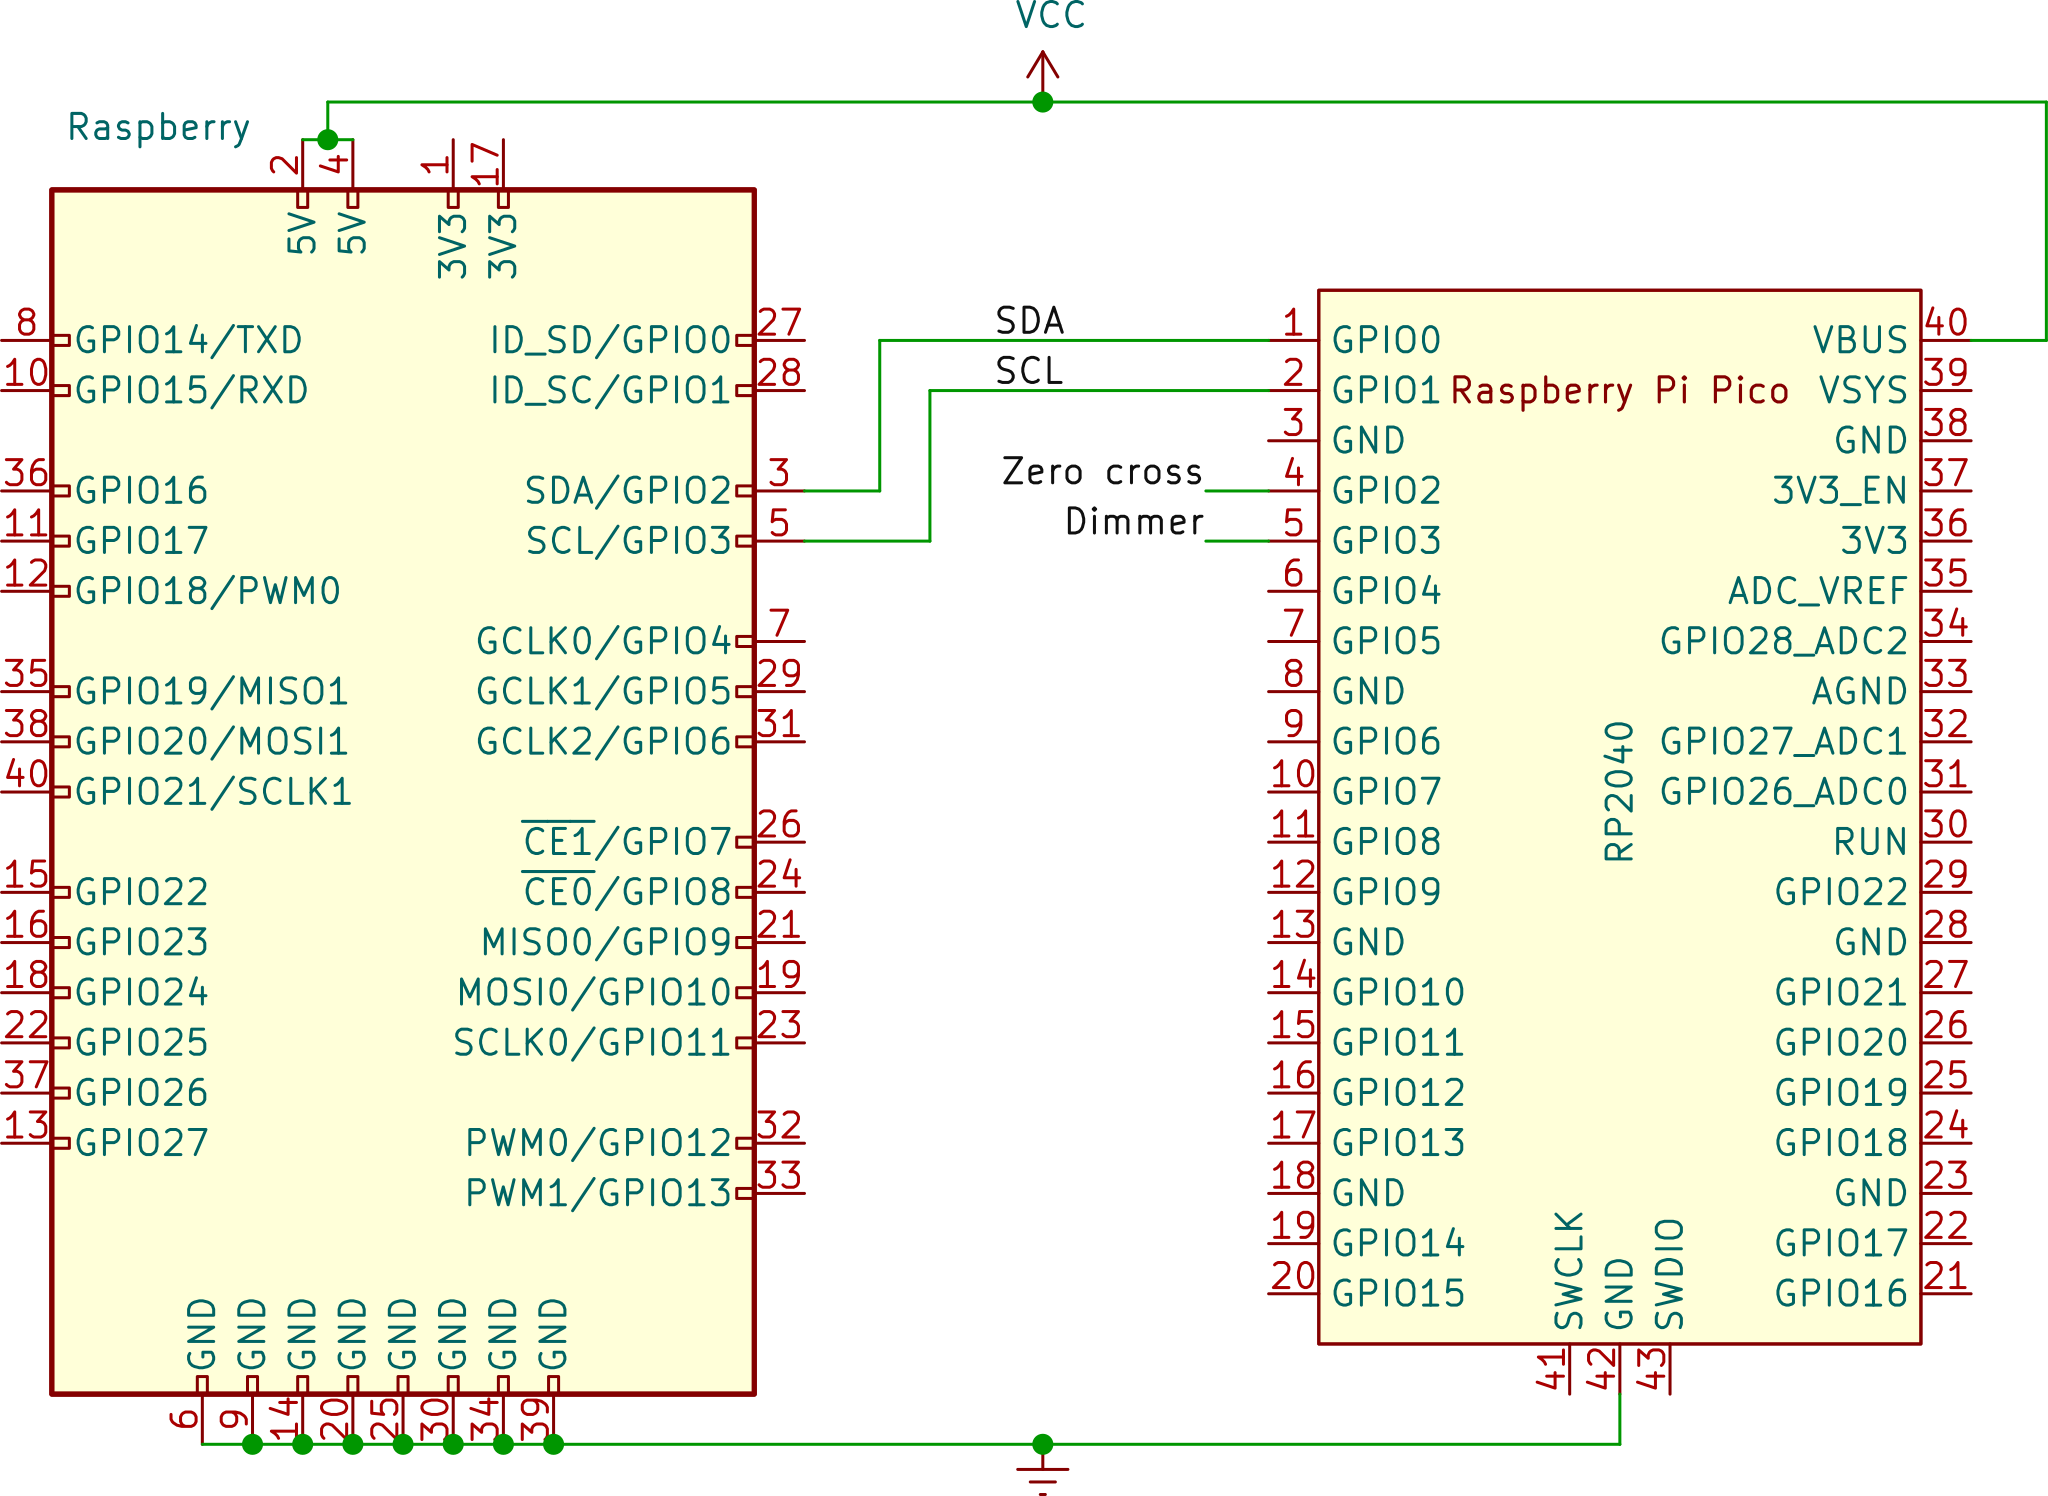
\includegraphics[width=0.5\columnwidth,height=7cm,keepaspectratio]{img/circuit-dc.png}
	\caption{Circuito de control en DC}%
	\label{fig:circuit-dc}
\end{figure}


\begin{table}
	\centering
	\caption{Conexiones \IIC entre Raspberry Pi y un Arduino}
	\label{tbl:pi-arduino-i2c} % CHKTEX 24
	\begin{tabularx}{0.8\linewidth}{cc rcl c c}
	\toprule
	\multicolumn{2}{c}{   Pin   } & \multicolumn{3}{c}{\multirow{2}{*}{Conexión}}  &     Pin     &     Pin     \\
	\multicolumn{2}{c}{Raspberry} & \multicolumn{3}{c}{}                           & Arduino UNO & Arduino Mega \\
	\midrule
	       3 & (GPIO2)            & Raspberry Pi SDA & \(\rightarrow{}\) & Arduino SDA & A4          & SDA (PIN 20) \\
	       5 & (GPIO3)            & Raspberry Pi SCL & \(\rightarrow{}\) & Arduino SCL & A5          & SCL (PIN 21) \\
	       6 & (\GND)             & Raspberry Pi GND & \(\rightarrow{}\) & Arduino GND & \GND        & \GND         \\
	\bottomrule
	\end{tabularx}
\end{table}

Esto es posible debido a que el Arduino no tiene resistencias de acoplamiento a positivo o \emph{pull-up} integradas, mientras que los pines \IIC de la Raspberry Pi están conectados internamente a la línea de 3.3V mediante resistencias de 1.8k\(\Omega{}\).
Por este motivo, tendrán que quitarse las resistencias de \emph{pull-up} a cualquier otro dispositivo esclavo que se conecte al bus \IIC de la Raspberry Pi.\footnote{Para más información sobre el papel de las resistencias de acoplamiento a positivo o \emph{pull-up} en un bus \IIC se puede consultar \url{http://dsscircuits.com/articles/effects-of-varying-i2c-pull-up-resistors} }

\medskip

A continuación pruebe el alambrado del circuito de DC con el programa de prueba del \Cref{sec:appendix1}.
El programa es muy simple, pues sólo configura interrupciones y cambia el estado de los pines cuando estas se producen.

\lstinputlisting[%
	language=C,
	caption={\texttt{arduino-code-i2c.cpp:14} --- Dirección asignada al dispositivo esclavo},
	label={lst:arduino-code-i2c-def},
	firstline=14,
	lastline=14]{src/arduino-code-i2c.cpp}

Al terminar el alambrado debería tener completo el citcuito de la \Cref{fig:circuit-full}
\begin{figure}[H]
	\centering
	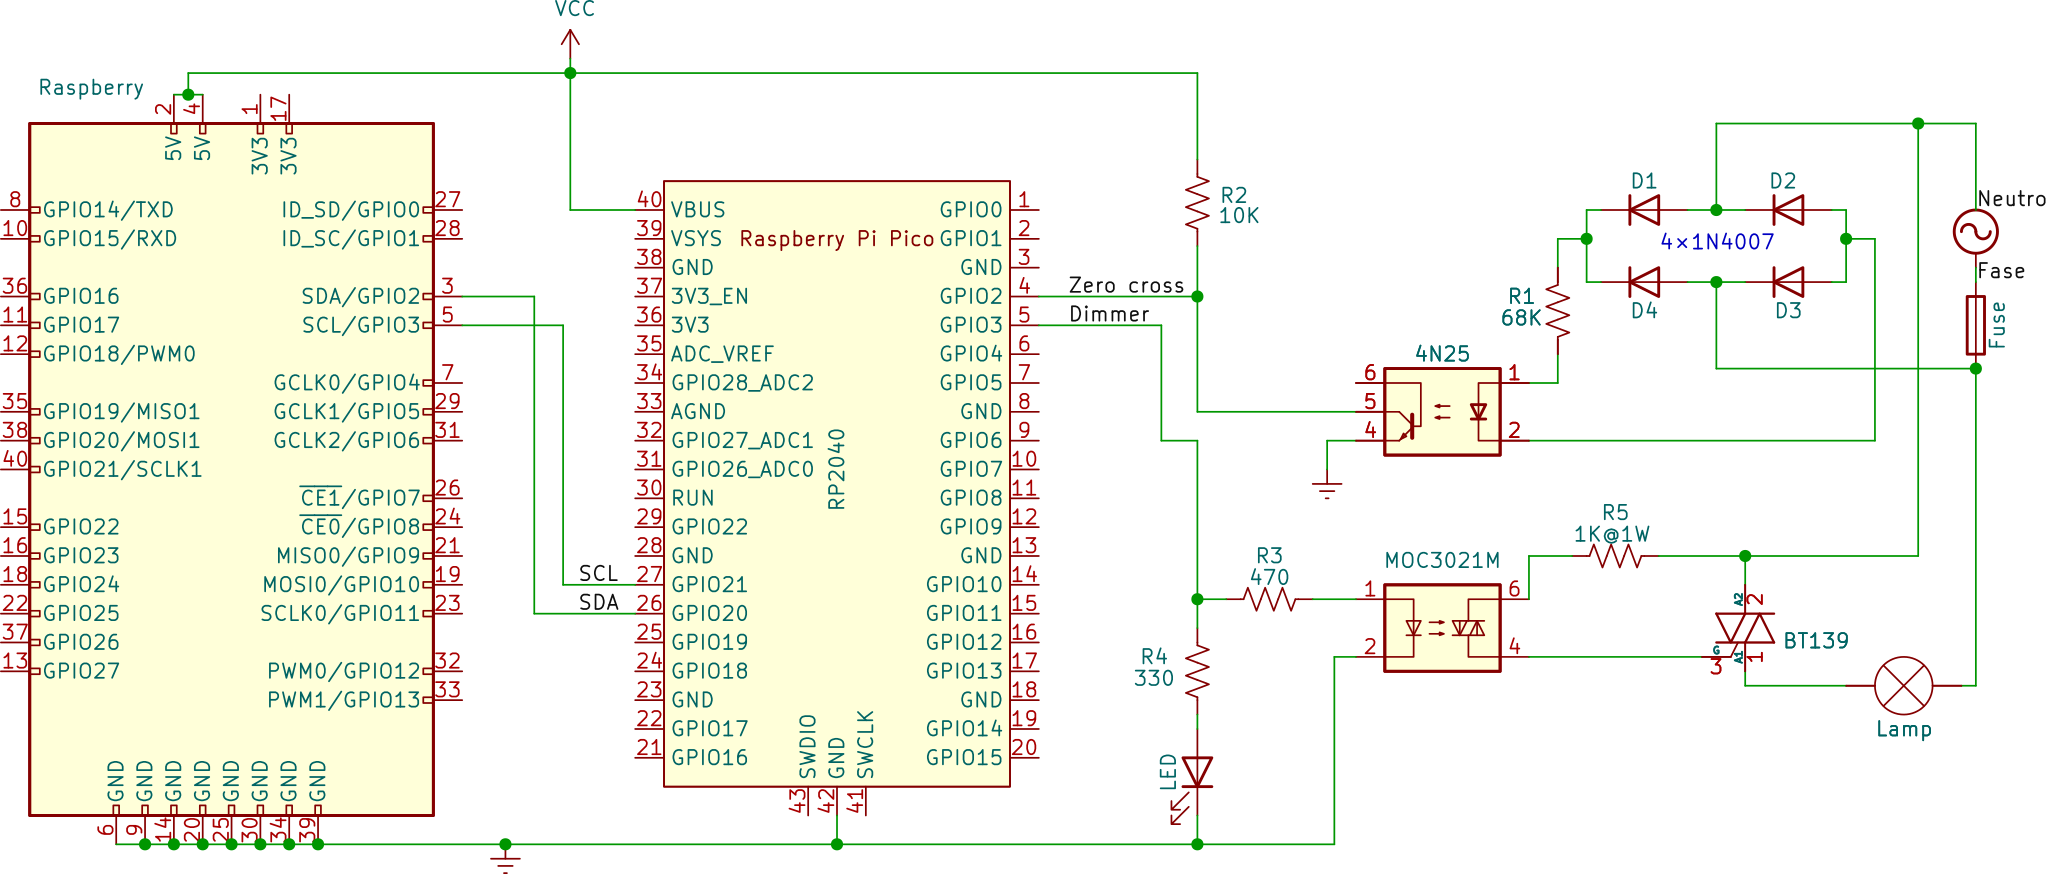
\includegraphics[width=0.75\columnwidth,height=9cm,keepaspectratio]{img/circuit-full.png}
	\caption{Diagrama de circuito alambrado completo}%
	\label{fig:circuit-full}
\end{figure}
